% Digital Logic Report Template 
% Created: 2020-01-10, John Miller

%==========================================================
%=========== Document Setup  ==============================

% Formatting defined by class file
\documentclass[11pt]{article}

% ---- Document formatting ----
\usepackage[margin=1in]{geometry} % Narrower margins
\usepackage{booktabs} % Nice formatting of tables
\usepackage{graphicx} % Ability to include graphics

%\setlength\parindent{0pt} % Do not indent first line of paragraphs 
\usepackage[parfill]{parskip} % Line space b/w paragraphs
% parfill option prevents last line of pgrph from being fully justified

% Parskip package adds too much space around titles, fix with this
\RequirePackage{titlesec}
\titlespacing\section{0pt}{8pt plus 4pt minus 2pt}{3pt plus 2pt minus 2pt}
\titlespacing\subsection{0pt}{4pt plus 4pt minus 2pt}{-2pt plus 2pt minus 2pt}
\titlespacing\subsubsection{0pt}{2pt plus 4pt minus 2pt}{-6pt plus 2pt minus 2pt}

% ---- Hyperlinks ----
\usepackage[colorlinks=true,urlcolor=blue]{hyperref} % For URL's. Automatically links internal references.

% ---- Code listings ----
\usepackage{listings} % Nice code layout and inclusion
\usepackage[usenames,dvipsnames]{xcolor} % Colors (needs to be defined before using colors)

% Define custom colors for listings
\definecolor{listinggray}{gray}{0.98} % Listings background color
\definecolor{rulegray}{gray}{0.7} % Listings rule/frame color

% Style for Verilog
\lstdefinestyle{Verilog}{
language=Verilog, % Verilog
backgroundcolor=\color{listinggray}, % light gray background
rulecolor=\color{blue}, % blue frame lines
frame=tb, % lines above & below
linewidth=\columnwidth, % set line width
basicstyle=\small\ttfamily, % basic font style that is used for the code 
breaklines=true, % allow breaking across columns/pages
tabsize=3, % set tab size
commentstyle=\color{gray}, % comments in italic 
stringstyle=\upshape, % strings are printed in normal font
showspaces=false, % don't underscore spaces
}

% How to use: \Verilog[listing_options]{file}
\newcommand{\Verilog}[2][]{%
\lstinputlisting[style=Verilog,#1]{#2}
}




%======================================================
%=========== Body  ====================================
\begin{document}

\title{ELC 4396 02 \\ Class Report 2}
\author{David Davis}

\maketitle


\section*{Introduction} 

The purpose of this class project was to get familiar with working with Verilog implementing more functions, such as button control, timers, and state machines. State machines were the main logic implemented in this project. The code would move from state to state to accomplish its function and display the results. The project was to build a system on the Nexys4 DDR board where the user would have three buttons to press that would allow the user to test their reflexes. When the user starts the system, an LED would light up after a certain period of time, and then the user would have to press a different button to stop the timer. \\\\GitHub Repo: \url{https://github.com/davisdavid/SoC}.


\section*{Implementation}

The first step in the process was to create a timer module. It would be implemented to count up in two different sections. The first would be the waiting period between when the user pressed the "start" button and then beginning of the test. Then the other section where the timer would be implemented is when the LED turns on and the timer is displayed on the seven segment display in milliseconds. The timer can be reset to start it over, allowing it to be used in multiple areas. The code for the timer module is shown below. 

\begin{lstlisting}[style=Verilog,caption=Timer Module ,label=code:ex ]
 module ms_timer(
    input logic clk,
    input logic rst,
    output logic [15:0] ms_ticks
    );
    
    output logic [31:0] count,
    logic [31:0] ncount;
    logic [15:0] ms_next;
    parameter MS = 20'b00011000011010100000;
    
    
    always_ff @(posedge clk, posedge rst)
      if(rst)
            begin
            count <=0; 
            ms_ticks <= 0;
            end
        else
            begin
            count<=ncount;
            ms_ticks <= ms_next;
            end
        
    always_comb
        if(count != MS)
            begin
            ncount = count + 1;
            ms_next = ms_ticks;
            end
        else if(count == MS)
            begin
            ms_next = ms_ticks + 1;
            ncount = 0;
            end
    
    
endmodule
\end{lstlisting}

The next module created was the binary to decimal converter (BDC). The decimal version of the time it took to stop the test would be needed to display on the seven segment display. This was done by splitting the 16 bit binary value into four sections and moving the values to correspond with decimal values.  This made the work much easier in the state machine button module. 

\begin{lstlisting}[style=Verilog,caption=Binary to Decimal Converter Module ,label=code:ex ]
module BDC(
    input logic [15:0] binary,
    output logic [3:0] thousands,
    output logic [3:0] hundreds,
    output logic [3:0] tens,
    output logic [3:0] ones
    );
    
    integer i;
    always_comb
    begin
        thousands = 4'd0;
        hundreds = 4'd0;
        tens = 4'd0;
        ones = 4'd0;
        
        for(i=15; i>=0; i--)
        begin
        //Add 3 to those > 5, to convert base 16 to base 10 after shift (+6)
            if(thousands >= 5)
                thousands+=3;
            if(hundreds >= 5)
                hundreds+=3;
            if(tens >= 5)
                tens+=3;
            if(ones >= 5)
                ones+=3;
            //Shift Left
            thousands = thousands << 1;
            thousands[0] = hundreds[3];
            hundreds = hundreds << 1;
            hundreds [0] = tens[3];
            tens = tens << 1;
            tens[0] = ones[3];
            ones = ones << 1;
            ones[0] = binary[i];
        end
    end
endmodule
\end{lstlisting}


The third module and largest module implemented was the state machine button module. This module contained the majority of the logic of the system using state machines. It contained six states for the system: INIT, WAITING, TOO\_EARLY, ON, TOO\_LATE, and COMPLETE. The init stage would display "HI" on the display and wait for the "start" button to be pressed. Once the "start" button was pressed, the timer would be reset, the display would be cleared, and the current state would move to the WAITING state. The WAITING state contained the code that controlled the time before the test would begin. The system would switch states if the random value assigned between two and fifteen seconds had been reached. If the "stop" button was pressed during this stage, "9999" would come on the display, the current state would move to the TOO\_EARLY state, and the system would have to be "cleared" to restart. Otherwise, the current state would move to the ON state. During the ON state, the LED would turn on, and the display would show the time in milliseconds. The system would move to the COMPLETE or TOO\_LATE state, depending on the response of the user. If the user pressed the "stop" button before the timer reached one second, the time at that instance would be saved and the current state would move to the COMPLETE state. Otherwise, the current state would move to the TOO\_LATE state. In the TOO\_LATE state, the value "1000" would show on the display and the system would have to be cleared to restart it. In the COMPLETE state, the saved time would be displayed and the LED would turn off. The system could then be cleared to restart the process. The code is shown below. 

\begin{lstlisting}[style=Verilog,caption=State Machine Button Module ,label=code:ex ]
module stateMachineButton(
    input logic clk,
    input logic rst,
    input logic btnu, btnc, btnd,
    output logic [15:0] display,
    output logic led2
    );
    
    logic db_btnu, db_btnc, db_btnd;
    logic manual_reset;
    logic [15:0] ms_ticks, decimal, stop_time;
    logic [31:0] random_value;
    int count;
    
    typedef enum logic [2:0] { INIT, WAITING, TOO_EARLY, ON, TOO_LATE, COMPLETE} State;
    State state, nstate;
    
    db_fsm mydb_btnu(
    .clk(clk),
    .reset(rst),
    .sw(btnu),
    .db(db_btnu)
    );
    
    db_fsm mydb_btnc(
    .clk(clk),
    .reset(rst),
    .sw(btnc),
    .db(db_btnc)
    );
    
    db_fsm mydb_btnd(
    .clk(clk),
    .reset(rst),
    .sw(btnd),
    .db(db_btnd)
    );
    
    ms_timer timer(
    .clk(clk),
    .rst(manual_reset),
    .ms_ticks(ms_ticks)
    );
    
    BDC myBDC(
    .binary(ms_ticks),
    .thousands(decimal[15:12]),
    .hundreds(decimal[11:8]),
    .tens(decimal[7:4]),
    .ones(decimal[3:0])
    );
    
    parameter ZERO   = 4'b0000;
    parameter ONE    = 4'b0001;
    parameter TWO    = 4'b0010;
    parameter THREE  = 4'b0011;
    parameter FOUR   = 4'b0100;
    parameter FIVE   = 4'b0101;
    parameter SIX    = 4'b0110;
    parameter SEVEN  = 4'b0111;
    parameter EIGHT  = 4'b1000;
    parameter NINE   = 4'b1001;
    parameter H      = 4'b1010;
    parameter I      = 4'b1011;
    parameter BLANK  = 4'b1100;
    
    always_ff @(posedge(clk), posedge(rst))
        if(rst)
            state <= INIT;
        else
            state <= nstate;     
    
    always_comb @(posedge(clk))
    case(state)
    INIT:
        begin
        led2 = 0;
        display = {BLANK, BLANK, H, I};
        if(btnu)
            begin
            manual_reset = 1;
            nstate = WAITING;
            random_value = $urandom_range(2,15);
            random_value = random_value * 1000;     
            end
        end
        
   WAITING:
        begin
        manual_reset = 0;
        display = {BLANK, BLANK, BLANK, BLANK};
        if(ms_ticks >= random_value)
            begin
            manual_reset = 1;
            led2 = 1;
            nstate = ON;
            end
        if(btnc)
            nstate = TOO_EARLY;
        if(btnd)
            nstate = INIT;    
        end         
        
    TOO_EARLY:
        begin
        display = {NINE, NINE, NINE, NINE};
        if(btnd)
        nstate = INIT;   
        end
        
    TOO_LATE:
        begin
        display = {ONE, ZERO, ZERO, ZERO};
        if(btnd)
        nstate = INIT;
        end
        
    ON:
        begin
        manual_reset = 0;
        display = decimal;
        if(btnc)
            begin
            stop_time = decimal;
            led2 = 0;
            nstate = COMPLETE;
            end
        if(btnd)
            nstate = INIT;
        if(ms_ticks >= 1000)
            nstate = TOO_LATE;       
        end 
        
    COMPLETE:
        begin
        display = stop_time;
        if(btnd)
        nstate = INIT;
        end      
    endcase
      
endmodule
\end{lstlisting}

The next step was to create the seven segment decoder. The seven segment decoder would just take the values passed to it from the state machine button module to make them appear on the display. The code was very simple so it wasn't embedded in this report. 


The seven segment driver from the last class report was also implemented that just turned on the correct anodes to display the values in the correct positions. 


The last step in the lab was to put all of the modules together in the main module. 

\section*{Results}
The lab was executed just like the prompt said it should be. The buttons functioned properly, the timer would count up correctly, and the the displays would show correctly. The video attached to this assignment shows the system functioning properly. 

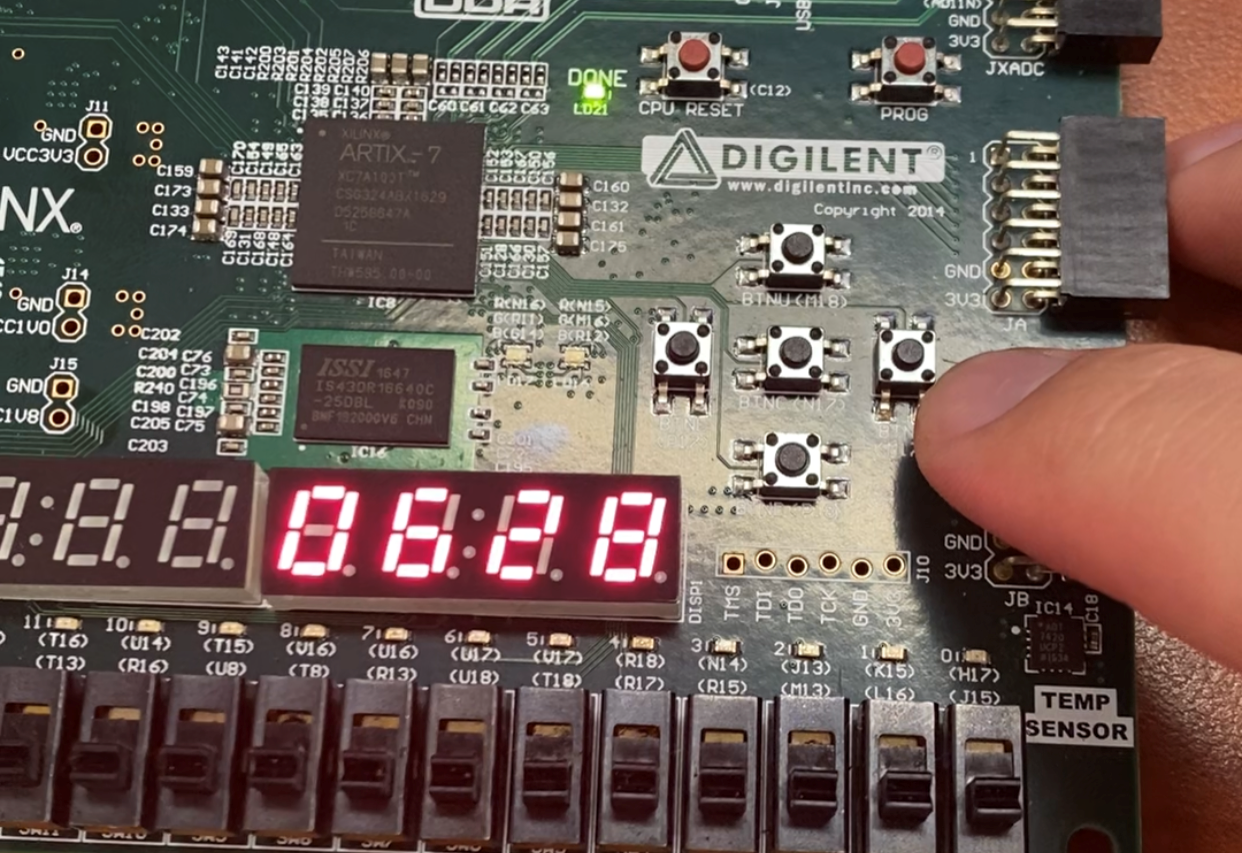
\includegraphics[height=.5\linewidth]{CR2pic.png}
\section*{Conclusion}

The project was very successful in implementing more functions like the timer and state machines. The state machines made up the majority of the logic in this lab, which made the code very readable and easy to understand. It was also beneficial in learning to connect different modules together to create a system. 


\end{document}